
\documentclass [11pt]{report}

\usepackage{fancyhdr}
\usepackage [french]{babel}

\usepackage[utf8]{inputenc}
\usepackage[T1]{fontenc}
\usepackage{textcomp}
\usepackage{graphicx}
\usepackage[a4paper]{geometry}
\usepackage{titlepic}
\usepackage{boxedminipage}
\usepackage{listings}
\usepackage{minitoc}
\usepackage{footmisc}
\usepackage{color}
\usepackage{graphicx}
\usepackage{fancyvrb}

\usepackage{eso-pic}

\makeatletter
\newlength\@tempdim@x
\newlength\@tempdim@y
% structure des commandes :
%   #1 = deplacement selon x
%   #2 = deplacement selon y
%   #3 = texte à mettre
\newcommand\AtUpperLeftCorner[3]{%
\begingroup
\@tempdim@x=0cm
\@tempdim@y=\paperheight
\advance\@tempdim@x#1
\advance\@tempdim@y-#2
\put(\LenToUnit{\@tempdim@x},\LenToUnit{\@tempdim@y}){#3}%
\endgroup
}
\newcommand\AtUpperRightCorner[3]{%
\begingroup
\@tempdim@x=\paperwidth
\@tempdim@y=\paperheight
\advance\@tempdim@x-#1
\advance\@tempdim@y-#2
\put(\LenToUnit{\@tempdim@x},\LenToUnit{\@tempdim@y}){#3}%
\endgroup
}
\newcommand\AtLowerLeftCorner[3]{%
\begingroup
\@tempdim@x=0cm
\@tempdim@y=0cm
\advance\@tempdim@x#1
\advance\@tempdim@y#2
\put(\LenToUnit{\@tempdim@x},\LenToUnit{\@tempdim@y}){#3}%
\endgroup
}
\newcommand\AtLowerRightCorner[3]{%
\begingroup
\@tempdim@x=\paperwidth
\@tempdim@y=0cm
\advance\@tempdim@x-#1
\advance\@tempdim@y#2
\put(\LenToUnit{\@tempdim@x},\LenToUnit{\@tempdim@y}){#3}%
\endgroup
}
% ajout de texte ou d'images en haut à gauche, en haut à droite, etc.
\AddToShipoutPicture{%
\AtLowerRightCorner{3cm}{1cm}{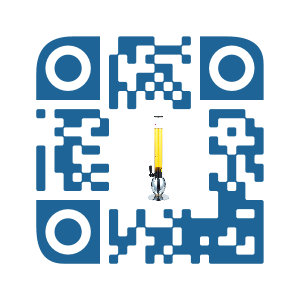
\includegraphics[scale=0.20]{images/LogoGroupe.png}}% image en bas à droite
}
\makeatother

\pagestyle{fancy}





\title{
	
\includegraphics[scale=0.43]{images/Logojeu.png}
	 \\\vspace{20mm}
	\textbf{\Huge \itshape Rapport de seconde soutenance  }
	}




\author{ \\\vspace{2mm}
	Thibault Gdalia\\\vspace{2mm}
	Florent Youinou\\\vspace{2mm}
	Mathilde Laplaze\\\vspace{2mm}
	Vincent Baille \\\vspace{30mm}
	}


\date{17 janvier 2014}


\usepackage{listings,mdframed,xcolor}
\definecolor{codeBackground}{rgb}{0.95, 0.95, 0.95} %Couleur du rectangle%


\lstnewenvironment{mylisting}{
  \lstset{
  }
  \mdframed[backgroundcolor=codeBackground,shadow=false,shadowsize=2pt,shadowcolor=black!30]
}
{
  \endmdframed\ignorespaces
}


\begin{document}
\thispagestyle{fancy}
\renewcommand{\baselinestretch}{0.001}
\maketitle
\tableofcontents

\chapter*{Introduction} 
Dans le cadre de notre premi\`ere année d'étude \`a EPITA, nous avons un projet informatique \`a réaliser tout au long du deuxi\`eme semestre. Nous sommes au milieu de la période prévu pour la réalisation de notre jeu. \\

Notre groupe de projet est toujours au complet, personne n'a quitté l'école depuis la derni\`ere soutenance. Petit Rappel, notre équipe est composée de 4 membres: Mathilde "Mattou" Laplaze, Florent "T4ze" Youinou, Vincent "Vincae" Baille et Thibault "Skeat" Gdalia. Lors de ce deuxi\`eme rapport, nous allons voir les différentes évolutions que nous avons apportées au jeu. Nous commencerons tout d'abord par rappeler ce que nous avions lors de la premi\`ere soutenance, l'état du moteur physique, les différents mode de jeu et l'éditeur de maps. \\

Depuis la premi\`ere soutenance nous avons modifiés l'ensemble des \'el\'ements existants dans le projet, car ce que nous avions \'et\'e bien mais pas suffisant pour pouvoir ajouter du nouveau contenu. Nous avons ajouter des nouveaut\'es, il nous manquait encore un mode de jeux complet, qui est imp\'eratif d'avoir pour pouvoir estimer avoir un jeux complet.\\





\chapter{Ce que nous avions}
	\section{Les différents mode de jeu}
		Lors de la soutenance précédente, deux modes de jeu étaient disponibles: le mode story et le mode infini.
		
		\vspace{10mm}
		
		\subsection{Story}
			Dans le mode story, une unique map était disponible. Ainsi vous deviez parcourir cette map jusqu'à la ligne d'arrivée pour gagner. De plus, si par malheur vous sortiez de l'écran par la gauche \`a-force de vous cogner contre des blocs ou pour une autre raison, vous aviez perdu et vous eties bon pour recommencer. Ce type de partie n'était pas trés intéressant car lorsque vous finissiez la map, vous aviez fini ce mode de jeu. \\
			
			\vspace{10mm}
			
			
			
			\subsection{Infini}
			Ce mode de jeu est lég\`rement différent, bien que la façon de jouer reste la m\^eme, le but du jeu differe legerement. Dans ce mode-ci, il n'y a pas de monde \`a valider puisqu'il n'y a tout simplement pas de fin. Le but est donc evidemment d'aller le plus loin possible. Une des particularitée de ce mode est que si l'on a deja cree un compte sur le site web officiel du jeux : www.CandyBird.eu, il nous est possible de nous connecter depuis le menu principal. Suite a cette connexion, notre score sera automatiquement envoye en ligne sur notre page de Classement (si vous avez fais un meilleur score que le precedent evidemment).\\
			
			Lors de notre premiere version du jeux, les blocs present sur la map etait généré de facon aleatoire tout en suivant un pourcentage fixe. Le probleme est que, avec cette implementation, le mode infini devenait vraiment complique puisque certains passages etait tout bonnement impossible a franchir. 
			
			\vspace{10mm}
			
	\section{Moteur physique}
		\indent Le Moteur physique était assez rudimentaire lors de la premi\`ere soutenance, lorsque l'on appuyait sur la barre espace l'oiseaumontait \`a vitesse constante. Sinon, le personnage redescendait tranquillement en planant \`a l'aide de ses petites ailes, toujours \`a la meme vitesse. Cela formait des trianglesEn cr\'ant les lois physique de notre jeu nous n'avions pas anticip'e le fait que nous voudrions le changer. C'est principalement pour cette raison que nous avions décidé de refaire intégralement le moteur physique, nous entrerons dans les détails de ces modifications plus tard dans ce rapport, dans la partie des modifications.\\
		
		\indent Il y avait également quelques probl\`emes dans certains cas de collision, que n'avions pas pris en compte. Par exemple lorsque l'oiseau touchait un bloc de face et qu'il avait un bloc au-dessus de lui, il était possible de traverser les blocs, ce probl\`eme permettait au joueur de tricher et d'éviter de mourir.\\
		
		\vspace{10mm}
		
		
	\section{Site internet}
		Notre site internet était déj\`a en ligne lors de la premi\`ere soutenance, et il était assez bien complet. vous pouvez y trouver la description de notre projet, une courte  présentation de chaque membre de l'équipe ainsi que quelques photos du jeu. Sur la page de télécharchement, vous pouvez récupérer notre cahier des charges et le rapport de la soutenance 1. Sur notre site vous avez egalement la possibilite de vous inscrire si vous voulez par la suite vous connecter au jeu. Pour finir, une page de classement des joueurs vous permet de comparer votre score avec les autres. 
		\vspace{10mm}
		
	\section{Graphismes}	
		Lors de la soutenance précédente nous avions déj\`a un grand nombre de graphisnes disponibles, tels que les fonds des menus, les sprites de l'oiseau, les différents boutons du jeux ainsi que les boutons de l'éditeur de maps. Nous avons créé un univers coloré autour de notre projet, ceci n'a pas changé depuis nous gardons toujours cette positions.
		
		\vspace{10mm}
		
	\section{Son}
		Nous avions déjà, lors de la première soutenance, des musiques differentes en fonction de l'état de jeu. Nous en modifierons sûrement quelques unes, mais cela n'est pas essentiel au projet. C'est pourquoi nous nous pencherons sur ce détail lorsque tout le reste sera termin\'e.\\
		\indent Le plus important actuellement est de rajouter des sons au cours du jeu : peur les collisions, pour les moment où la barre de vie est trop basse ou qu'elle augmente grâce à un bonbon.. Mais encore une fois, nous nous pencherons sur ce travail plus tard car nous pensons \`a rajouter encore différents types de bonbons, ou des bonus.
		
		\vspace{10mm}


	\section{\'Editeur de maps}
		L'éditeur était un élément un peu a part dans notre projet. Nous nous en étions pas énormément servi pour la soutenance précédente, car nous l'avions terminer un peu tardivement, et que le projet n'était pas suffisamment avancé pour nous en ayons réellement besoin.
		
		
		\vspace{10mm}
		
		
\chapter{Les modifications}
	\section{Mode de Jeu}
		Pour cette seconde soutenance, les deux modes de jeux existants ont été modifié.
		Il était nécessaire d'améliorer ces modes, aussi bien pour rallonger la durée de vie du jeux, que pour l'embellir et le rendre plus agréable à jouer.
		\vspace{10mm}
		\subsection{Story}
			Nous avons donc modifié notre mode histoire afin qu'il ressemble plus a ce que l'on a l'habitude de trouver dans la plupart des jeux.\\
			
			\indent Pour commencer, nous avons rajout\'e des niveaux. Nous avons donc mis en place un menu vous permettant de choisir le niveau, et donc la map sur laquelle vous voulez jouer, à condition bien s\^ur de l'avoir débloquée en arrivant au moins une fois à bout du niveau précédent. Il y a aujourd'hui neuf maps disponibles o\`u la difficulté augmente au fur et à mesure que l'on avance dans les niveaux. \`A l'aide de l'éditeur de map, il n'a pas été compliqué de créer chaque map et cela a nous a fait gagné pas mal de temps, car nous avons décidé de faire des maps d'une longueur de 500 blocs de long, c'est \`a dire que sur chaque ligne il peut y avoir potentiellement 500 blocs sur chaque ligne, ce qui n'arrive pas car cela ne représente pas un réel intérêt pou le jeux. Cependant, cette t\^ache n'a pas \'et\'e instantanée car nous voulions avoir des maps qui représentent un certain challenge. La création de maps était la partie la moins intéressante de la préparation de la soutenance. C'est pour cela nous nous y sommes donc mis tous ensemble pour venir à bout de ce travail.\\
			
			Par la suite, chaque membre du groupe a testé les différentes maps pour vérifier quelles soient toutes jouables sans qu'elles soient trop simple : il serait dommage d'avoir du contenu qui ne soit pas exploitable par le joueur.\\
			
			
			\newpage
			
			\indent Afin d'étoffer notre projet, nous avons fait quelques niveaux avec des propriétés particulières. Par exemple, dans le monde 8, la gravité est inversée. Dans le monde 5, certains blocs se détruisent au contact de l'oiseau, en lui faisant baisser sa barre de vie. Cela apporte une difficulté en plus, et nous en rajouterons probablement d'autres plus tard. Cette initiative nous a amenés à travailler à nouveau sur les collisions, ainsi que sur le moteur physique. En effet, il fallait forcement pouvoir adapter ces deux derniers afin de les rendre modulables en fonction de la map jouée.	
					
			\vspace{6mm}				
			\begin{figure}[h]
				\centering
				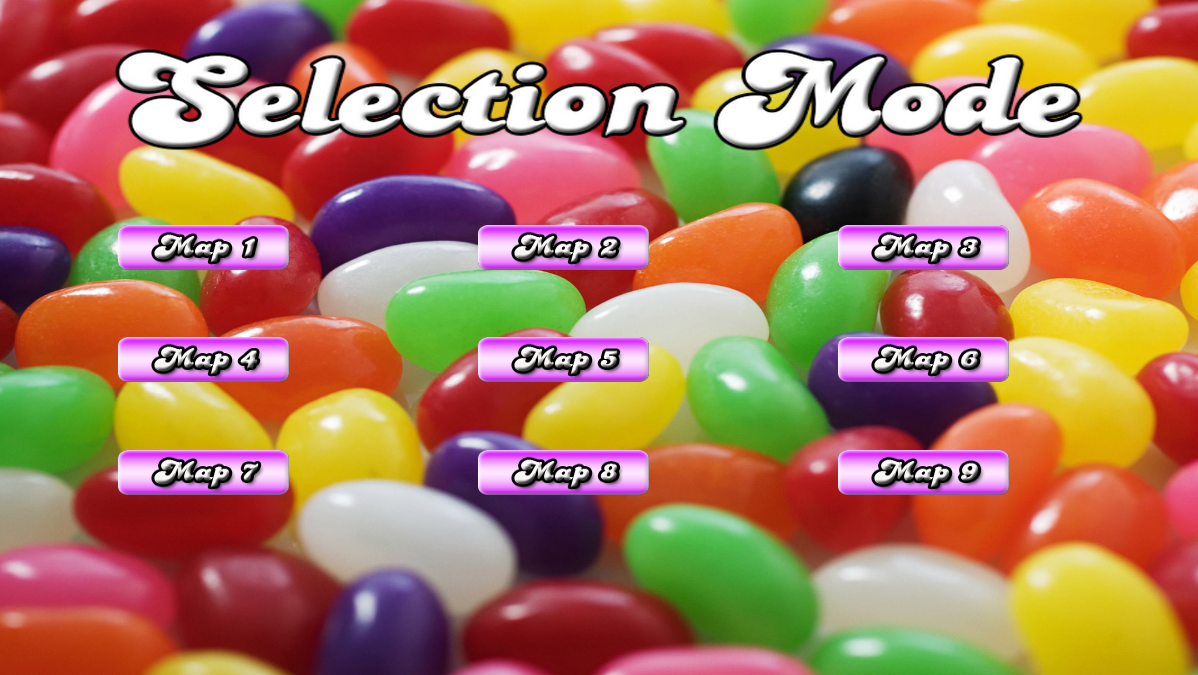
\includegraphics[width=0.7\linewidth]{images/map_menu.png}
				\caption[Map Menu]{Choix de Maps}				
				\label{fig:Map Menu}
			\end{figure}
			\vspace{10mm}
			
		\subsection{Infini}
			Le mode Infini est une des plus grosses parties du jeu car c'est en générale ce que les utilisateurs préfèrent. Etant nous même des utilisateurs potentiels de CandyBird, nous savons que le système de comparaison de score sur le site est très apprécié.
						
			Lors de la dernière soutenance nous avions déjà bien avancé. Nous avons tout de même modifié les apparitions aléatoire des blocs car ce mode manquait d'harmonie.\\
						
						
			Cette nouvelle version est beaucoup plus "logique" en terme de jouabilité. Puisque le problème était l’enchaînement des blocs, pourquoi ne pas rendre cette génération standard afin de régler cette génération quasi impossible a franchir. Nous avons donc choisit de préparer de nombreux patterns, tous de même longueur, commençant et se terminant toujours par les mêmes blocs. Ainsi c'est l’enchaînement des pattern qui se fait de façon aléatoire et le map infini crée reste tout a fait jouable. En faite ce principe suit le même principe que si les différents mondes s’enchaînaient infiniment et de façon aléatoire les uns après les autres, sauf que ce ne sont pas les mêmes mondes.\\
			
			Nous avons créé plusieurs patterns, qui s'enchainent aléatoirement. Nous avons estimé que 7 patterns suffisaient pour le moment. La création de pattern se fait de la même façon que les maps. Encore une fois l'éditeur de map nous a pas mal servi. La création de patterns a \'et\'e aussi longue que la création de maps.\\
			
			
			\begin{figure}[h]
				\centering
				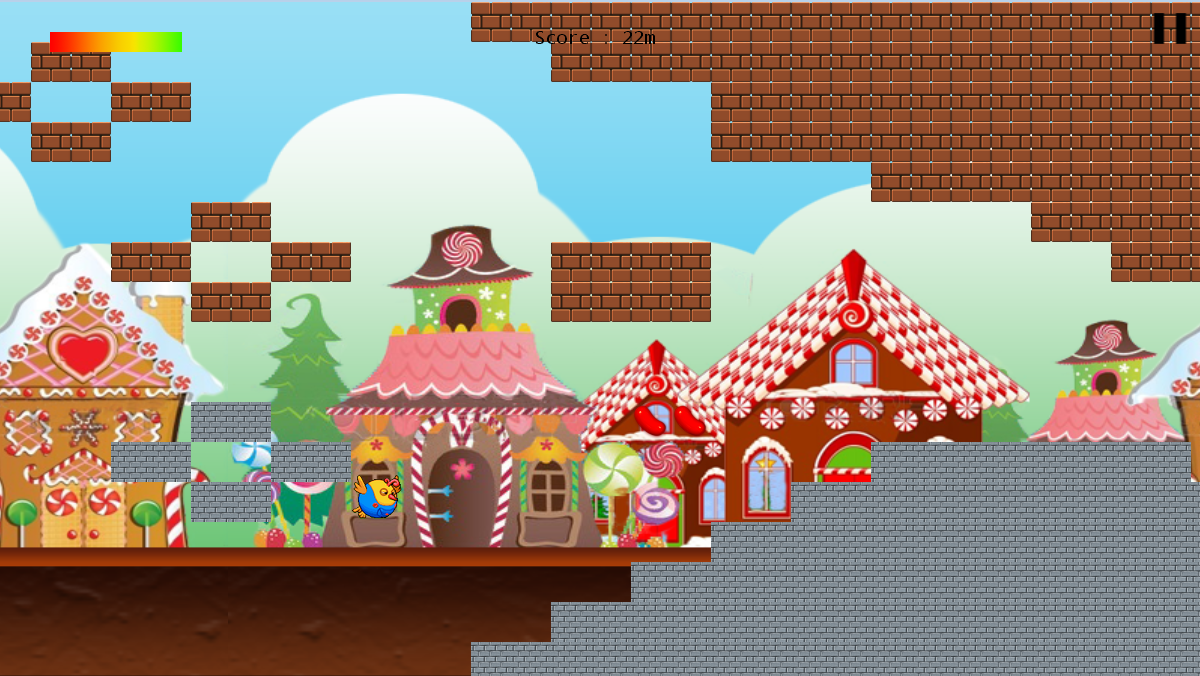
\includegraphics[width=0.7\linewidth]{images/pattern.png}
				\caption[Editeur de Maps]{exmples de patterns}	
				\label{fig:Pattern}
			\end{figure}
						
			Par la suite il nous suffira de rajouter des patterns et des bonus afin d'augmenter la diversité des décors et la jouabilité.
			
			\vspace{10mm}
			
\newpage
	\section{Moteur Physique}
		Depuis la dernière soutenance nous avons complètement revue le moteur physique. Nous nous sommes fait la remarque qu'un jeu bas\'e sur un oiseau qui vole nécessite un bon moteur physique. C'est donc Mattou qui s'est attelée \`a cette t\^ache. \\
		
		Elle a commencé en modifiant le code initial, mais les problèmes s'accumulaient et elle n'arrivait pas \`a tous les arranger. Elle a donc fini par prendre la décision de repartir de zéro. Cela lui a fait perdre du temps, mais pas en vain car le jeu possède maintenant un moteur physique qui lui donne un effet plus r\'ealiste. En effet, au lieu de simplement monter et descendre avec une vitesse constante, il saute maintenant en suivant une certaine accélération qui simule les propri\'et\'es physiques d'un corps en chute libre. Cela donne donc au joueur une impression de gravit\'e. Mattou a \'egalement fait attention \'a ce que le nouveau moteur physique soit facilement adaptable \'a des propri\'et\'es physiques plus particuli\`res, pour pouvoir faire varier la difficult\'e d'un niveau \`a un autre. Le moteur physique du jeu a donc \'et\'e nettement am\'elor\'e. \\
		
		\indent Une fois que nous avons jugé la trajectoire de l'oiseau satisfaisante, il a fallu se pencher sur les collisions. Comme dit précédemment, elles ne fonctionnaient pas toutes parfaitement. Et nous ne pouvions pas nous contenter de réparer les erreurs à-partir du code existant, car étant donné les modifications au niveau du mode histoire, il nous fallait un code modulable et facile à adapter à chaque niveau.\\
		
		\noindent Par exemple :\\
		\indent\indent - Pour le niveau 8, les collisions ne sont pas gérées de la meme manière car si l'oiseau touche un bloc qui est en-dessous de lui, il ne doit pas pouvoir se poser étant donné que le centre de gravité est au-dessus de lui.
		
		\indent\indent - Pour le niveau 5, les blocs n'empêchent pas forcément l'oiseau d'avancer en fonction de leur nature. Certains disparaissent seulement, et affaiblissent l'oiseau.\\
		
		
		Tous ces détails demandent un moteur physique adapté pour chaque map. Nous avons donc maintenant des collisions qui fonctionnent toutes sans exception.
		
		\vspace{10mm}
		
	\section{Editeur de Maps}
		Nous avons apporté quelques modifications a notre éditeur de maps car nous n'avions pas encore vu ses limites, tout d'abord il fallu tout d'abord revoir l'initialisation de la map, car nous étions bloqué avec une longueur de 100 cubes dans la longueur, ce qui rendait les parties trés courtes, aujourd'hui il est possible de créer des maps d'une longueur de 1 000 cubes par lignes, ce qui est largement suffisant pour le moment car les maps que nous créons pour le mode story sont d'une longueur de 500 cubes par lignes, nous estimons que cela est largement suffisant pour que le joueur puisse s'amuser.\\
				
		\indent Nous avons aussi du revoir le chargement des maps existantes. En effet, lors de la soutenance précédente nous n'avions pas pensé a ce genre d'utilisation. Il s'avère que cela est très pratique lors des tests des nouvelles maps car au début nous ne pouvions rien faire si la map se trouvait \^etre infaisable. En réalité nous pouvions modifier, en ouvrqnt la maps sur un éditeur de texte tel que notepad et changer la valeur de la case \`a la main, mais cette solution n'était pas envisageable \`a grande échelle. C'est pourquoi nous avons incorporé une fonction permettant de charger des maps dans l'éditeur de maps afin de les modifier aussi facilement qu'on les créer.\\
		
		\begin{figure}[h]
			\centering
			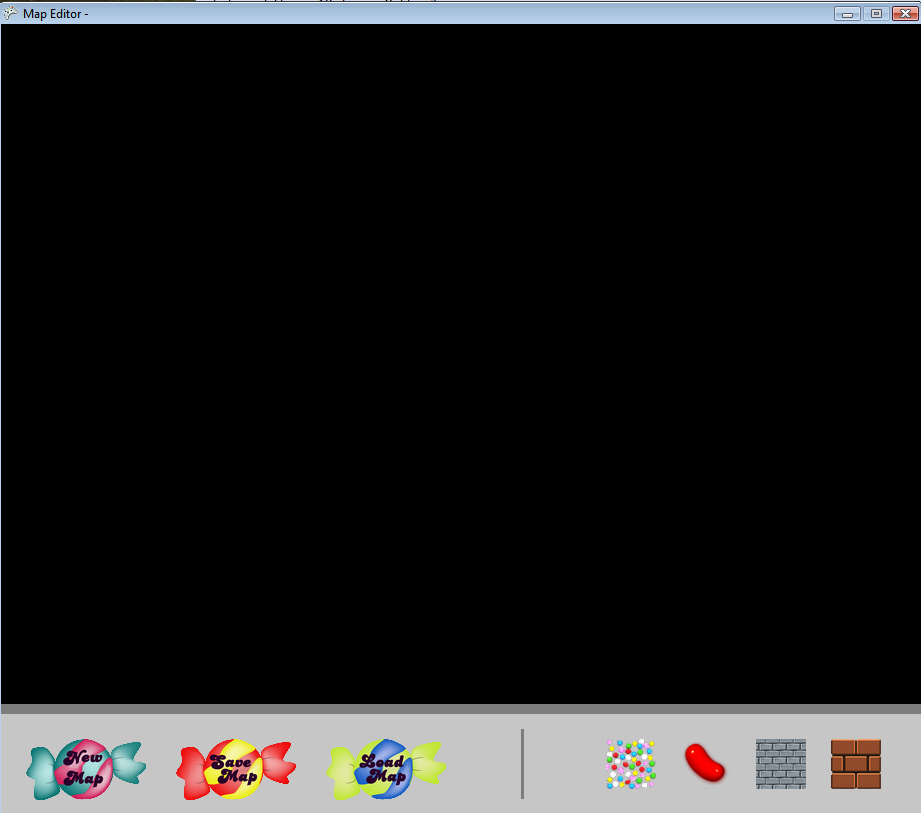
\includegraphics[width=0.7\linewidth]{./images/Editeur}
			\caption[Editeur de Maps]{Editeur de Maps}
			\label{fig:Editeur}
		\end{figure}
		\vspace{10mm}
		
		
\chapter{Les nouveautés}
	\section{Le Réseau}
		Pouvoir jouer seul en débloquant des niveaux, jouer dans un mode infini et repousser ses limites et même envoyer son score en ligne sont des possibilités intéressantes. Mais à part comparer son score, on se sens vite seul, et on peux se lasser du jeux. En restant dans la même optique, si vous êtes à plusieurs, vous n'avez pas forcement envie de jouer chacun votre tour, cela créer des tensions.\\
		
		C'est pourquoi nous avons choisit, pour votre plus grand plaisir, d'apporter une "légère" nouveauté à CandyBird : Un réseau.\\
		
		Grâce à se réseau, finit les prises de têtes pour savoir à qui est-ce le tour de jouer, vous pourrez tous jouer en même temps !
		Le but de notre réseau n'est pas d'arriver avant les autres au bout de la map comme dans la plupart des courses que l'on connait. D'ailleur vous pouvez toujours essayer d'arriver avant les autres mais le mode infini n'as pas de fin donc cela va être compliqué.. De plus, la map défile à la même vitesse et les blocs s'enchainent de la même façon chez toutes les personnes connectée au même server. Vous devez donc survivre aussi longtemps que les autres, et être le dernier en vie pour faire le meilleur score. Tout comme donc le mode infini normal, votre score est envoyer sur notre site en cas de défaite, afin que votre meilleur score soit sauvegardé.\\
		
		A l'instar du jeux Trackmania ou le but est de faire le meilleur temps même si les voitures ne commencent pas toutes en même temps, ici il faut allez le plus loin possible. On rappel que votre score est traduit sous forme d'un compteur de mètres dans la partie supérieur de CandyBird.
		
		\newpage
		
		\subsection{Comment l'utiliser ?}
		\vspace{6mm}
		\begin{center}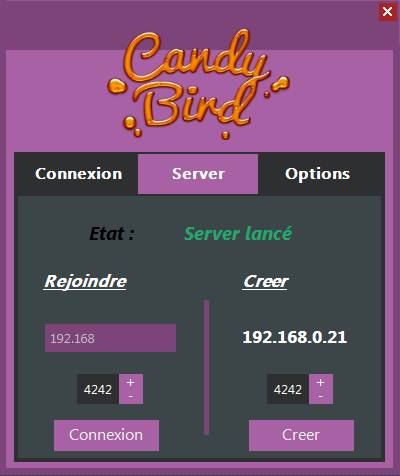
\includegraphics[scale=0.43]{images/panel.jpg}\end{center}
		\vspace{6mm}
				
		Disponible depuis le nouveau panel de connexion, dans le second onglet intitulé "server", vous avez désormais le choix entre rejoindre ou créer un server. Dans le premier cas, il vous suffira de rentrer l'adresse ip ainsi que le port sur lequel est exécuté le server. Dans le second, seul le port est nécessaire et vous pourrez ensuite partager les informations à vos amis pour qu'ils s'y connecte à leur tour. Pour l'aspect visuel du mode réseau, vous pouvez également, dans le troisième onglet, sélectionner la couleur de vos adversaires. En effet si tout le monde est de la même couleur sur la map, on ne sait plus qui est qui..\\		
		
		Maintenant que vous êtes connecté au server, le votre ou celui d'un ami, ce que vous souhaitez,  c'est pouvoir jouer ! Et bien il suffit simplement de lancer le mode infini et vous verrez votre/vos amis apparaitre sur la map à vos cotés.\\		
				
		\vspace{10mm}
		
		
		\subsection{Comment le réseau s'est construit ?}
		
		Aucun membre du groupe n'avait de connaissance en réseau, il a donc fallut se lancer dans des recherches afin de comprendre comment faire. C'est T4ze qui s'est occupé d'implémenter les parties correspondantes à ce réseau. En y reflechissant, une analogie avec un chat lui est venu à l'esprit. En effet, dans un chat il y a un server principal et les messages de chaque personne sont envoyé à tous le monde. Ici, dans CandyBird c'est exactement ce que nous voulons, sauf qu'à la place des messages, ce sont des positions qui sont envoyées.\\
		
		Pour ne pas s'embrouiller dans le code, il a décider de créer dans un premier temps un projet externe contenant ce "Chat". Après avoir passé tous nos test et s'être avéré être une solution viable, ce projet secondaire à été intégré au projet principal.\\
		
		Lorsque vous créez le server, c'est une application externe qui se lance. De cette façon, si le server rencontre un problème, que la connexion lâche ou qu'un quelconque problème survient, le jeux ne risque rien. \\
				
		La première version du server marchait parfaitement mais il y avait un léger problème. On voyait clairement les différents joueurs se déplacer sur la carte mais la génération de map était propre à chaque joueur, et donc personne n'avaient la même map et on voyait des joueurs traverser des blocs. Pour que chacun joue avec les mêmes blocs il a fallut rendre unique cette génération. Logiquement, c'est l'utilisateur qui héberge le server qui a ete choisit pour générer la map pour tous les autres.\\
				
		A chaque Update du Game1, les Clients envoie leur pseudo ainsi que leur position (sur x et sur y). De même, ils récupèrent les données envoyées par les autres Clients afin de mettre à jour leur position. Ainsi les joueurs apparaissent sur les écrans de tout le monde en temps réel.
		
		
		
				
		
	
	
\chapter{Avancement du Projet}
	\renewcommand{\arraystretch}{2}
	\setlength{\tabcolsep}{0.7cm}
	\begin{tabular}{|c|c|c|}
	\hline  & premi\`ere soutenance & deuxi\`eme soutenance\\ 
	\hline Moteur Physique & 50\% & 95\% \\ 
	\hline \'Editeur de maps & 60\% & 90\% \\ 
	\hline Son & 80\% & 85\% \\ 
	\hline Mode Histoire & 50\% &  80\%\\ 
	\hline Mode Infini & 50\% & 90\% \\ 
	\hline Réseau &  0\% & 90\% \\ 
	\hline Graphismes & 60\% & 60\% \\ 
	\hline Site internet & 80\% & 85\% \\ 
	\hline
	\end{tabular} 
	
	
	
	
\chapter{La suite}
	\section{Graphisme}
	\section{Editeur de map}
		Nous pensons ajouter directement notre éditeur de map a notre jeu dans le but de faciliter la possibilité pour le joueur de créer des maps. En effet jusqu'à présent nous étions obligés de lancer l'éditeur de map en dehors de notre jeu qui lui est pourtant entièrement dédié, cependant nous pensons qu'il serait plus simple pour le joueur de pouvoir accéder à l'éditeur directement depuis le jeu, sans avoir à passer par un autre logiciels complètement détaché de ce dernier. 
		
		
		
\chapter*{Conclusion}
	Tout au long de ce rapport, nous avons fait un point sur l'\'etat d'avancement du projet, les modifications, et les nouveaut\'ees. Nous pouvons voir que les bases ont \'et\'e consolid\'ees pour pouvoir supporter les \'evolutions que nous avons apport\'es au jeu et celles qui arriveront avant la fin de l'ann\'ee, peut-\^etre qu'il faudra encore les revoir, mais il y a tr\`es peu de chance que nous ayons besoin de tout restructurer comme nous venons de le faire. \\
	
	Les modifications apport\'ees aux mode de jeu Story et Infini Apporte un r\'eel plus \`a la jouabilit\'e du jeu, nous pensons ainsi que les futurs joueur du jeu seront appr\'eci\'es le travail fournit. Nous avons la dur\'ee de vie du mode story, et les mode Infini a reçu un r\'eel refondemment dans l'apparition de blocs, ce qui le rend plus jouable et plus agr\'eable.\\
	
	Le nouveau mode r\'eseau apporte une r\'eelle valeur ajout\'ee au projet, gr\^ace \`a lui nous pouvons esp\'erer toucher de plus en plus de joueur. L'\'elaboration de ce mode de jeu n'a pas \'et\'e une t\^ache facille mais nous y sommes parvenu.\\
	
	Aujourd'hui CandyBird, a un r\'eel moteur physique, diff\'erents mode jeu qui permet de r\'epondre au attentes d'un grand nombre de joueurs, le mode story permet de relever des d\'efis que notre groupe a pr\'epar\'e, chaque joueur peut montrer son niveau dans le jeu gr\^ace au mode infiny, et il est d\'esormais possible de s'amuser entre amis avec le nouveau mode r\'eseau.\\
	
	Tout le travail apport\'e sur le projet, nous a permis de bien avanc\'e, nous sommes satisfait par le r\'esultat que tout cela donne. De plus quand nous faisons le point sur le planning que nous avons \'etabli dans le cahier des charges, nous sommes dans les temps 
\end {document}